\section{Reducing The Branching Factor}
The branching factor associated with each tile on the perimeter of an empty room (in an 8-connected 
grid map) is dependent on the dimensions of the room.
Consider an empty room of width $w$ and height $h$ where $w > h$.
After adding all non-dominated macro edges, each tile has (depending on its position on the perimeter) 
between $h$ and $2h - 1$ neighbours from the opposite side 
of the room. 
In addition, each tile has up to 4 other neighbours from elsewhere on the perimeter of the same room and
up to 3 neighbours located in an adjacent room.
Thus the total branching factor can be as high as $2h + 6$.
Generally speaking, a linear branching factor is undesirable as invididual node expansion operations 
take longer and additional neighbours usually add more branches to the search tree and make it more 
difficult to reach the goal.
\par
We will address this problem in two ways: (i) by reducing the number of tiles that must be evaluated during search and 
(ii) by attempting to reduce the branching factor directly.
The first method is an offline technique that prunes tiles from the perimeter of each empty room. 
The second is an online pruning strategy which we apply during individual node expansions.
We will discuss both methods in the context of 8-connected grid maps however
they are equally applicable to 4-connected grid maps also.
\par \noindent \newline
\textbf{Perimeter Reduction:}
We observe that in many cases there are tiles on the perimeter of an empty room which have no neighbours from any 
adjacent room. 
These tiles represent intermediate locations between entry and exit points that lead into and out of each empty room.
To speed up search we propose pruning from the perimeter of each room all such nodes.
To preserve optimality, we will connect the neighbours of each pruned node directly to each other.
The weight of each new edge is therefore equal to the octile distance between the two neighbours.
Figure \ref{fig-branching} (Top) shows an example.
This is a very simple optimisation but as we will see, it can have a dramatic effect on the average performance of
A* on certain types of maps.

\begin{figure}[t]
       \begin{center}
                       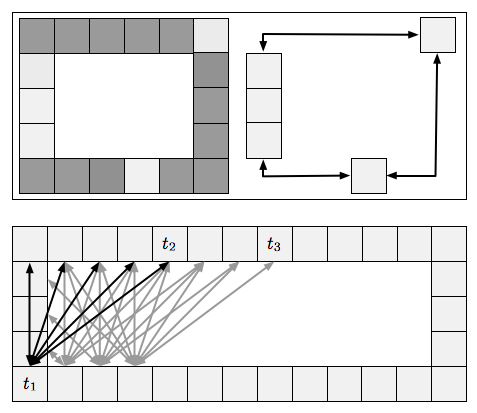
\includegraphics[scale=0.5, trim = 10mm 10mm 10mm 0mm]{diagrams/branching.png}
       \end{center}
	\vspace{-3pt}
       \caption{(Top) From each empty room we prune all (dark grey) tiles which have no neighbours in any adjacent room. 
Remaining tiles are then connected directly.
\\
		(Bottom) A path enters an empty room at tile $t_{1}$ and exits at tile $t_{3}$. Notice that once
$t_{1}$ is expanded we generate $t_{2}$. The edge ($t_{1}$, $t_{2}$) is an optimal traversal to the opposite side of the room.
This allows us to ignore all secondary neighbours of nodes descended from $t_{1}$ in the search
tree (e.g $t_{4}, t_{5}, t_{6}$).
}
       \label{fig-branching}
\end{figure}

\par \noindent \newline
\textbf{Faster Node Expansion:} 
Ensuring optimality during search requires connecting each tile on the perimeter
of an empty room to a linear number of neighbours on the opposite side of the
room.
This is undesirable as each node expansion then becomes a linear time operation. 
%By comparison, on an unmodified 8-connected grid map, each node expansion takes constant time.
We will improve this situation by developing a node expansion strategy which can, in many cases, skip all neighbours from 
the opposite side of the room (and therefore run in constant time).
Our strategy is straightforward; an example is given in Figure
\ref{fig-branching} (Bottom):

%We can improve this situation by observing that when the search enters an empty room an optimal length path to a node on
%the opposite side of the room is immediately found.
%of the room is immediately found.
%Any subsequent node expansions cannot possibly improve the length of this path, we propose skipping all such neighbours.

\begin{enumerate}
\item{Divide the set of neighbours associated with each tile on the perimeter of an empty room into two distinct sets:
\emph{primary neighbours} and \emph{secondary neighbours}.
Secondary neighbours are those which are located on the opposite side of the
room to the current tile  (excluding any corner tiles).
Primary neighbours are all the rest.}
\item{During node expansion, determine which room the parent of the current node belongs to.}
\item{If the parent and the current node belong to different rooms (or if the current node has no parent) 
process all primary and secondary neighbours.
However, if the parent and the current node belong to the same room, process only primary neighbours.}
\end{enumerate}

\begin{lemma}
The ``Fast Node Expansion'' strategy preserves optimality during search.
\end{lemma}
\begin{proof}
We just provide a proof sketch. 
Let $m$ be a node on the perimeter of a room. Assume that its parent $p$ belongs
to the same room.
Let $n$ be a secondary successor of $m$.
Recall that $n$ and $m$ are on opposite sides of the room.
We argue below that passing through $m$ cannot possibly improve the 
best path between $p$ and $n$.
Therefore, there is no need to consider $(m,n)$ macro-edges
when $m$ and $p$ belong to the same room.

There are four cases when a node $m$ and its parent $p$ belong to the
same room. In case 1, $p$ is the start node and is placed inside the room.
Obviously, the path segment $p,m,n$ is suboptimal, as we zigzag from $p$ to one
edge and then to the opposite edge of the room.
In cases 2, 3, and 4, $p$ and $m$ are on opposite edges, on ortoghonal edges, and on the same
edge, respectively. As in case 1, it is possible to check in each case that
taking a detour through $m$ does not improve the shortest path between $p$ and $n$.
\end{proof}

%Let $R$ be an empty room in an 8-connected grid map.
%Further, let $m$ and $n$ be two arbitrarily selected tiles from the perimeter of $R$.
%There are three cases to consider when searching for an optimal path between $m$ and $n$:
%\begin{enumerate}
%\item{$m$ and $n$ are on the same side of the room.}
%\item{$m$ and $n$ are on orthogonal sides of the room.}
%\item{$m$ and $n$ are on opposite sides of the room.}
%\end{enumerate}
%In all cases we begin by expanding $m$ and process all its primary and secondary neighbours.
%In the first and second case the optimal path from $m$ to $n$ involves no tiles from the opposite side of the room;
%the decision to ignore all secondary neighbours has no effect on the optimality of the solution.
%In the third case we argue as follows:
%when we expand $m$ we generate a node $n'$ on the same side of the perimeter as $n$.
%The edge $(m, n')$ represents a path that crosses the room from $m$ to $n'$
%using a maximum number of diagonal steps. 
%From this it is trivial to derive that the path $\lbrace m, n', n \rbrace$ is itself optimal.
%Thus we can ignore all secondary neighbours of nodes descended from $m$ in the search tree
%(evaluating them could not possibly improve the length of any path from $m$ to $n$).
%\end{proof}
%%It is worth noting that on 4-connected maps the branching factor of each tile on
%%the perimeter is already constant. 
%%Applying Fast Node Expansion in this case often results in an average branching
%%factor smaller than 4. 
%%On 8-connected maps the effectiveness of this approach is dependent on how well
%%we can decomposde the grid map into large rectangular rooms.



